
% This LaTeX was auto-generated from MATLAB code.
% To make changes, update the MATLAB code and republish this document.

\documentclass{article}
\usepackage{graphicx}
\usepackage{color}

\sloppy
\definecolor{lightgray}{gray}{0.5}
\setlength{\parindent}{0pt}

\begin{document}

    
    
\subsection*{Contents}

\begin{itemize}
\setlength{\itemsep}{-1ex}
   \item Unknown Input Observer Dynamic System Matricies
   \item Simulation results
   \item Sim the system
\end{itemize}


\subsection*{Unknown Input Observer Dynamic System Matricies}


\begin{verbatim}The coupled mass-spring system is a well studied mechanical setup in
control theory.  Here we develop an UIO for this system under
disturbances.
Author: Sam Nazari
Date:  April 2015\end{verbatim}
    \begin{verbatim}
clear,clc
\end{verbatim}
\begin{verbatim}
%----------System Parameters---------%
k   = 1   %
m   = 1   % kg
c   = 1 %
\end{verbatim}

        \color{lightgray} \begin{verbatim}
k =

     1


m =

     1


c =

     1

\end{verbatim} \color{black}
    \begin{verbatim}
%----------State Space Formulation---------%
A   = [0 0 1 0;
       0 0 0 1;
       -2*k/m k/m -c/m 0;
       k/m -2*k/m 0 -c/m]

B   = [0;0;0;k/m]
C   = [1 0 0 0;0 1 0 0;0 0 1 0;0 0 0 1]
D   = 0
E   = [0;0;0;1]
\end{verbatim}

        \color{lightgray} \begin{verbatim}
A =

     0     0     1     0
     0     0     0     1
    -2     1    -1     0
     1    -2     0    -1


B =

     0
     0
     0
     1


C =

     1     0     0     0
     0     1     0     0
     0     0     1     0
     0     0     0     1


D =

     0


E =

     0
     0
     0
     1

\end{verbatim} \color{black}
    \begin{verbatim}
%----------LQR Control---------%
Q=[100 0 0 0;
    0 100 0 0;
    0 0 100 0;
    0 0 0 100]
R=1
[Klqr ll ss]=lqr(A,B,Q,R)
\end{verbatim}

        \color{lightgray} \begin{verbatim}
Q =

   100     0     0     0
     0   100     0     0
     0     0   100     0
     0     0     0   100


R =

     1


Klqr =

   -1.3620   10.4615    2.0165   10.0419


ll =

  162.7361  -21.0481   23.8552   -1.3620
  -21.0481  133.5821   25.6448   10.4615
   23.8552   25.6448   71.8220    2.0165
   -1.3620   10.4615    2.0165   10.0419


ss =

  -9.7953 + 0.0000i
  -0.6104 + 1.3684i
  -0.6104 - 1.3684i
  -1.0259 + 0.0000i

\end{verbatim} \color{black}
    \begin{verbatim}
%----------Step 1: rank(CE) = rank(E) ?= 1---------%
rank(C*E)
rank(E)
\end{verbatim}

        \color{lightgray} \begin{verbatim}
ans =

     1


ans =

     1

\end{verbatim} \color{black}
    \begin{verbatim}
%----------Step 2: Compute observer matrices---------%
H = E*inv((C*E)'*(C*E))*(C*E)'
T = eye(4)-H*C
A1 = T*A
\end{verbatim}

        \color{lightgray} \begin{verbatim}
H =

     0     0     0     0
     0     0     0     0
     0     0     0     0
     0     0     0     1


T =

     1     0     0     0
     0     1     0     0
     0     0     1     0
     0     0     0     0


A1 =

     0     0     1     0
     0     0     0     1
    -2     1    -1     0
     0     0     0     0

\end{verbatim} \color{black}
    \begin{verbatim}
%----------Step 3:Check (C,A1) rank---------%
rank(obsv(A1,C)) % Check observability of the pair (C,A1)
\end{verbatim}

        \color{lightgray} \begin{verbatim}
ans =

     4

\end{verbatim} \color{black}
    \begin{verbatim}
%----------Step 4: Choose observer poles---------%
K1 = place(A',C',[-2,-10,-5,-3])'
\end{verbatim}

        \color{lightgray} \begin{verbatim}
K1 =

     2     0     1     0
     0    10     0     1
    -2     1     4     0
     1    -2     0     2

\end{verbatim} \color{black}
    \begin{verbatim}
%----------Step 5: Finish observer design---------%
F = A1-K1*C
K = K1 + F*H
\end{verbatim}

        \color{lightgray} \begin{verbatim}
F =

    -2     0     0     0
     0   -10     0     0
     0     0    -5     0
    -1     2     0    -2


K =

     2     0     1     0
     0    10     0     1
    -2     1     4     0
     1    -2     0     0

\end{verbatim} \color{black}
    

\subsection*{Simulation results}

\begin{par}
Set up simulation initial condiditons
\end{par} \vspace{1em}
\begin{verbatim}
x1_0       = -1;
x2_0       = -5;
x3_0       = 1;
x4_0       = 1; % theta = pi is vertically upward equilibrium

% sim time
TSIM = 30

d=5   % time that disturbance occurs
\end{verbatim}

        \color{lightgray} \begin{verbatim}
TSIM =

    30


d =

     5

\end{verbatim} \color{black}
    

\subsection*{Sim the system}

\begin{verbatim}
sim('massSpringMDL')
figure,
plot(tout,X(:,1)-X_hat(:,1),'r'),hold on,
plot(tout,X(:,2)-X_hat(:,2),'b'),hold on,
plot(tout,X(:,3)-X_hat(:,3),'k'),hold on,
plot(tout,X(:,4)-X_hat(:,4),'g'),
title('State Estimation Error for coupled mass spring system')
xlabel('time (sec)'),ylabel('m and m/s')
legend('q_1','q_2','dq_1','dq_2','Location','NorthEast')
xlim([0,10])
ylim([-1,1])
\end{verbatim}

        \color{lightgray} \begin{verbatim}Warning: Using a default value of 0.6 for maximum step size.  The simulation
step size will be equal to or less than this value.  You can disable this
diagnostic by setting 'Automatic solver parameter selection' diagnostic to
'none' in the Diagnostics page of the configuration parameters dialog 
\end{verbatim} \color{black}
    
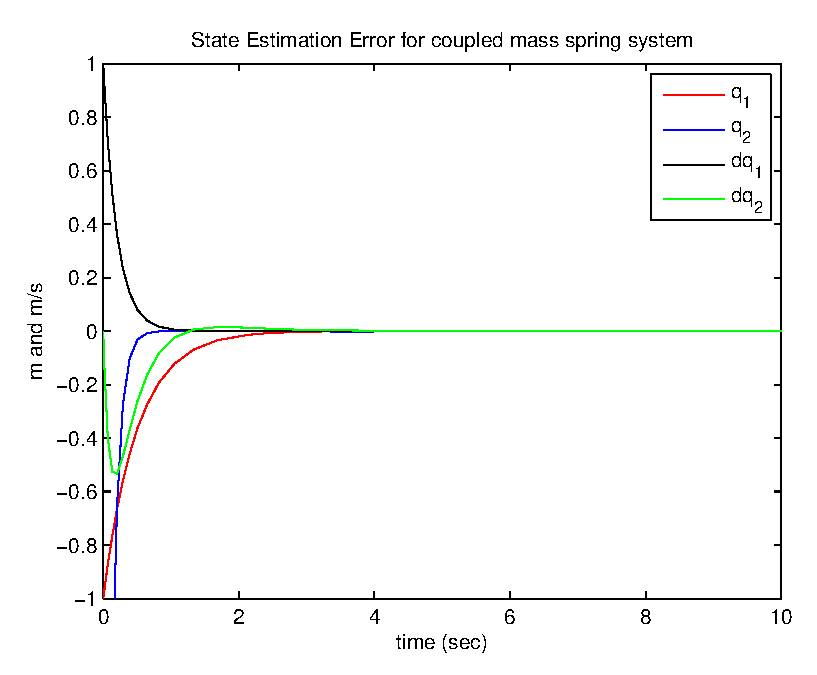
\includegraphics [width=4in]{massSpring_01.eps}



\end{document}
    
